%% LaTeX-Beamer template for KIT design
%% by Erik Burger, Christian Hammer
%% title picture by Klaus Krogmann
%%
%% version 2.1
%%
%% mostly compatible to KIT corporate design v2.0
%% http://intranet.kit.edu/gestaltungsrichtlinien.php
%%
%% Problems, bugs and comments to
%% burger@kit.edu

\documentclass[18pt, hideallsubsections, handout]{beamer}

\usepackage[utf8]{inputenc}
\usepackage{csquotes}

%% SLIDE FORMAT

% use 'beamerthemekit' for standard 4:3 ratio
% for widescreen slides (16:9), use 'beamerthemekitwide'
% for widescreen slide without sidebar use 'beamerthemekitwidenosidebar'

\usepackage{templates/beamerthemekitwide}
%\usepackage{templates/beamerthemekitwide}
%\usepackage{templates/beamerthemekitwidenosidebar}

% use this to disable the latex beamer navigation symbols
\beamertemplatenavigationsymbolsempty
\setbeamerfont{section in sidebar}{size=\fontsize{8}{8}\selectfont}


%% TITLE PICTURE

% if a custom picture is to be used on the title page, copy it into the 'logos'
% directory, in the line below, replace 'mypicture' with the
% filename (without extension) and uncomment the following line
% (picture proportions: 63 : 20 for standard, 169 : 40 for wide
% *.eps format if you use latex+dvips+ps2pdf,
% *.jpg/*.png/*.pdf if you use pdflatex)

%\titleimage{mypicture}

%% TITLE LOGO

% for a custom logo on the front page, copy your file into the 'logos'
% directory, insert the filename in the line below and uncomment it

%\titlelogo{mylogo}

% (*.eps format if you use latex+dvips+ps2pdf,
% *.jpg/*.png/*.pdf if you use pdflatex)

%% TikZ INTEGRATION

% use these packages for PCM symbols and UML classes
% \usepackage{templates/tikzkit}
% \usepackage{templates/tikzuml}

\usepackage{caption}
\usepackage{mathtools}
\DeclarePairedDelimiterX\set[1]\lbrace\rbrace{\def\given{\;\delimsize\vert\;}#1}
\newcommand\defas\coloneqq

\usepackage{tikz}
\usetikzlibrary{positioning}
\usetikzlibrary{arrows}
\usetikzlibrary{fit}
\usetikzlibrary{shapes}
\usetikzlibrary{calc}

\usetikzlibrary{arrows.meta}
\tikzset{
    every picture/.append style={
        >={Stealth[length=2mm]}
    }
}

% https://tex.stackexchange.com/questions/55806/mindmap-tikzpicture-in-beamer-reveal-step-by-step/55849#55849
\tikzset{
    invisible/.style={opacity=0},
    visible on/.style={alt={#1{}{invisible}}},
    alt/.code args={<#1>#2#3}{%
        \alt<#1>{\pgfkeysalso{#2}}{\pgfkeysalso{#3}} % \pgfkeysalso doesn't change the path
    },
}

% the presentation starts here

\title[Graphen III]{Graphen 3:\\ Maximum Flow, Bipartite Matching}
\subtitle{Ford-Fulkerson, Edmond-Karp, Max Flow, Min Cut, MCBM, Bipartite Graphen, Vertex Cover, König}
\author{Robert Brede, Peter Koepernik, Serge Thilges, Jean-Pierre von der Heydt}

\institute{Basispraktikum zum ICPC Programmierwettbewerb}

% Bibliography

\usepackage[citestyle=authoryear,bibstyle=numeric,hyperref,backend=biber]{biblatex}
\addbibresource{templates/example.bib}
\bibhang1em

\setbeamercovered{invisible}
\begin{document}

% change the following line to "ngerman" for German style date and logos
\selectlanguage{ngerman}

%title page
\begin{frame}
\titlepage
\end{frame}

%table of contents
%\begin{frame}{Gliederung}
%\tableofcontents
%\end{frame}

\section{Maximum Flow}
\tikzset{
  in place/.style={
    auto=false,
    fill=white,
    inner sep=2pt,
  },
}
  \tikzstyle{vertex}=[circle,fill=black!25,minimum size=20pt,inner sep=0pt]
  \tikzstyle{source}=[circle,fill=red!25, minimum size = 30pt, inner sep = 0pt]
  \tikzstyle{target}=[circle,fill=blue!25, minimum size = 30pt, inner sep = 0pt]
  \tikzstyle{edge} = [draw,thick,-]
  \tikzstyle{diredge} = [draw,thick,->]
  \tikzstyle{selected diredge} = [draw,thick,->,red]

  \subsection{Motivation}
  \begin{frame}{Beispielaufgabe}
    \setbeamercovered{invisible}
    \begin{block}{Beispielaufgabe}
      \begin{itemize}
        \item Gegeben sei ein Netz mit Städten und Straßen mit einer Kapazität
        \pause
        \item Für gewisse Städte A und D sucht man die Anzahl Autos die von A nach D fahren können
      \end{itemize}
    \end{block}
  \end{frame}
    \begin{frame}{Motivation}
  \setbeamercovered{invisible}
    
    \begin{figure}
        \begin{tikzpicture}[scale=2.3, auto,swap]
        \node[source] (A) at (0, 0) {A};
        \node[vertex] (B) at (1, -1) {B};
        \node[vertex] (C) at (1, 1) {C};
        \node[target] (D) at (2, 0) {D};
        
        
    % A - B
    \path[diredge]<1> (A) --  (0.4, -0.6);
    \path[diredge]<1> (0.4, -0.6) -- node[pos=0, in place] {70} (B);

    \path[diredge]<1-> (B) -- (0.6, -0.4);
    \path[diredge]<1-> (0.6, -0.4) --node[pos=0, in place] {70} (A);

    % A - C
    \path[diredge]<1-3> (A) -- (0.4, 0.6);
    \path[diredge]<1-3> (0.4, 0.6) -- node[pos=0, in place] {30} (C);

    \path[diredge]<1-> (C) -- (0.6, 0.4);
    \path[diredge]<1-> (0.6, 0.4) -- node[pos=0, in place] {30} (A);

    % C - D
    \path[diredge]<1-3> (C) -- (1.6, 0.6);
    \path[diredge]<1-3> (1.6, 0.6) -- node[pos=0, in place] {50} (D);

    \path[diredge]<1-> (D) -- (1.4, 0.4);
    \path[diredge]<1-> (1.4, 0.4) -- node[pos=0, in place] {50} (C);

    % B - D
    \path[diredge]<1> (B) -- (1.6, -0.6);
    \path[diredge]<1> (1.6, -0.6) -- node[pos=0, in place] {50} (D);
    
    \path[diredge]<1-> (D) -- (1.4, -0.4);
    \path[diredge]<1-> (1.4, -0.4) -- node[pos=0, in place] {50} (B);
    
    % B - C
    \path[diredge]<1-4> (B) -- (0.7,0);
    \path[diredge]<1-4> (0.7, 0) -- node[pos=0, in place] {15} (C);
    \path[diredge]<1-> (1.3,0) -- (B) ;
    \path[diredge]<1-> (C) -- node[pos=1, in place] {15} (1.3,0);
  

    \path[selected diredge]<2> (A) --  (0.4, -0.6);
    \path[selected diredge]<2> (0.4, -0.6) -- node[pos=0, in place] {70} (B);

    \path[selected diredge]<2> (B) -- (1.6, -0.6);
    \path[selected diredge]<2> (1.6, -0.6) -- node[pos=0, in place] {50} (D);

    \path[diredge]<3-4> (A) --  (0.4, -0.6);
    \path[diredge]<3-4> (0.4, -0.6) -- node[pos=0, in place] {20} (B);

    \path[diredge]<3-6> (B) -- (1.6, -0.6);
    \path[diredge]<3-6> (1.6, -0.6) -- node[pos=0, in place] {0} (D);
    
    \path[selected diredge]<4> (A) -- (0.4, 0.6);
    \path[selected diredge]<4> (0.4, 0.6) -- node[pos=0, in place] {30} (C);

    \path[selected diredge]<4> (C) -- (1.6, 0.6);
    \path[selected diredge]<4> (1.6, 0.6) -- node[pos=0, in place] {50} (D);

    % A - B
    \path[selected diredge]<5> (A) --  (0.4, -0.6);
    \path[selected diredge]<5> (0.4, -0.6) -- node[pos=0, in place] {20} (B);

    % A - C
    \path[diredge]<5-6> (A) -- (0.4, 0.6);
    \path[diredge]<5-6> (0.4, 0.6) -- node[pos=0, in place] {0} (C);

    % C - D
    \path[selected diredge]<5> (C) -- (1.6, 0.6);
    \path[selected diredge]<5> (1.6, 0.6) -- node[pos=0, in place] {20} (D);

    % B - C
    \path[selected diredge]<5> (B) -- (0.7,0);
    \path[selected diredge]<5> (0.7, 0) -- node[pos=0, in place] {15} (C);

    \path[diredge]<6> (B) -- (0.7,0);
    \path[diredge]<6> (0.7, 0) -- node[pos=0, in place] {0} (C);
    
    \path[diredge]<6> (A) --  (0.4, -0.6);
    \path[diredge]<6> (0.4, -0.6) -- node[pos=0, in place] {5} (B);

    \path[diredge]<6> (C) -- (1.6, 0.6);
    \path[diredge]<6> (1.6, 0.6) -- node[pos=0, in place] {15} (D);
          
           
    \end{tikzpicture}
  \end{figure}
  \begin{center}
    \pause \pause 50
    \pause \pause  + 30
    \pause  + 15 = 95
  \end{center}

  
\end{frame}

\subsection{Ford Fulkerson}
\subsubsection{Algorithmus}
\begin{frame}{Ford Fulkerson}
  \setbeamercovered{invisible}
  %\rightarrow
  \begin{block}{Ford Fulkerson}
    \begin{itemize}
      \item $F = 0$
      \pause
      \item Solange ein steigender Pfad p ($s \rightarrow\dots\rightarrow i$ $\rightarrow j\rightarrow\dots\rightarrow t$) von $s$ nach $t$ existiert:
      \pause
      \begin{itemize}
      \item 1. finde minimale Kante $f$ auf dem Pfad
      \pause
      \item 2. Kapazität aller Kanten in Pfadrichtung (z.B. $i\rightarrow j$) um $f$ reduzieren
      \pause
      \item 3. Kapazität aller Kanten gegen Pfadrichtung (z.B. $j\rightarrow i$) um $f$ erhöhen 
      \pause
      \item $F \mathrel{+}= f$;
      \end{itemize}
    \end{itemize}
  \end{block}
\end{frame}
\subsubsection{Rückkante}
\begin{frame}{Rückkante}
  \setbeamercovered{invisible}
  \begin{figure}
    \begin{tikzpicture}[scale=2.3, auto,swap]
    \node[source] (A) at (0, 0) {A};
    \node[vertex] (B) at (1, -1) {B};
    \node[vertex] (C) at (1, 1) {C};
    \node[target] (D) at (2, 0) {D};
    
    % A - B
    \path[diredge]<1> (A) --  (0.4, -0.6);
    \path[diredge]<1> (0.4, -0.6) -- node[pos=0, in place] {50} (B);

    \path[diredge]<1,2,6> (B) -- (0.6, -0.4);
    \path[diredge]<1,2,6> (0.6, -0.4) --node[pos=0, in place] {0} (A);

    % A - C
    \path[diredge]<1-4> (A) -- (0.4, 0.6);
    \path[diredge]<1-4> (0.4, 0.6) -- node[pos=0, in place] {50} (C);

    \path[diredge]<1-> (C) -- (0.6, 0.4);
    \path[diredge]<1-> (0.6, 0.4) -- node[pos=0, in place] {0} (A);

    % C - D
    \path[diredge]<1> (C) -- (1.6, 0.6);
    \path[diredge]<1> (1.6, 0.6) -- node[pos=0, in place] {50} (D);

    \path[diredge]<1,2,6> (D) -- (1.4, 0.4);
    \path[diredge]<1,2,6> (1.4, 0.4) -- node[pos=0, in place] {0} (C);

    % B - D
    \path[diredge]<1-4> (B) -- (1.6, -0.6);
    \path[diredge]<1-4> (1.6, -0.6) -- node[pos=0, in place] {50} (D);
    
    \path[diredge]<1-> (D) -- (1.4, -0.4);
    \path[diredge]<1-> (1.4, -0.4) -- node[pos=0, in place] {0} (B);
    
    % B - C
    \path[diredge]<1> (B) -- (0.7,0);
    \path[diredge]<1> (0.7, 0) -- node[pos=0, in place] {50} (C);
    \path[diredge]<1,2,6> (1.3,0) -- (B) ;
    \path[diredge]<1,2,6> (C) -- node[pos=1, in place] {0} (1.3,0);
  

    \path[selected diredge]<2> (A) --  (0.4, -0.6);
    \path[selected diredge]<2> (0.4, -0.6) -- node[pos=0, in place] {50} (B);

    \path[selected diredge]<2> (B) -- (0.7,0);
    \path[selected diredge]<2> (0.7, 0) -- node[pos=0, in place] {50} (C);
    
    \path[selected diredge]<2> (C) -- (1.6, 0.6);
    \path[selected diredge]<2> (1.6, 0.6) -- node[pos=0, in place] {50} (D);
  
    \path[diredge]<3-5> (B) -- (0.6, -0.4);
    \path[diredge]<3-5> (0.6, -0.4) --node[pos=0, in place] {50} (A);

    \path[diredge]<3> (1.3,0) -- (B) ;
    \path[diredge]<3> (C) -- node[pos=1, in place] {50} (1.3,0);
  
    \path[diredge]<3-5> (D) -- (1.4, 0.4);
    \path[diredge]<3-5> (1.4, 0.4) -- node[pos=0, in place] {50} (C);


    \path[diredge]<3-5> (A) --  (0.4, -0.6);
    \path[diredge]<3-5> (0.4, -0.6) -- node[pos=0, in place] {0} (B);
    
    \path[diredge]<3-5> (C) -- (1.6, 0.6);
    \path[diredge]<3-5> (1.6, 0.6) -- node[pos=0, in place] {0} (D);

    \path[diredge]<3> (B) -- (0.7,0);
    \path[diredge]<3> (0.7, 0) -- node[pos=0, in place] {0} (C);
      
    \path[diredge]<4-5> (B) -- (0.7,0);
    \path[diredge]<4-5> (0.7, 0) -- node[pos=0, in place] {0} (C);

    \path[diredge]<4> (1.3,0) -- (B) ;
    \path[diredge]<4> (C) -- node[pos=1, in place] {50} (1.3,0);

    \path[selected diredge]<5> (1.3,0) -- (B) ;
    \path[selected diredge]<5> (C) -- node[pos=1, in place] {50} (1.3,0);
    
    \path[selected diredge]<5> (A) -- (0.4, 0.6);
    \path[selected diredge]<5> (0.4, 0.6) -- node[pos=0, in place] {50} (C);

    \path[selected diredge]<5-6> (B) -- (1.6, -0.6);
    \path[selected diredge]<5-6> (1.6, -0.6) -- node[pos=0, in place] {50} (D);
    
    \path[diredge]<6> (B) -- (0.7,0);
    \path[diredge]<6> (0.7, 0) -- node[pos=0, in place] {50} (C);
    
    \path[diredge]<6> (1.3,0) -- (B) ;
    \path[diredge]<6> (C) -- node[pos=1, in place] {0} (1.3,0);
  

    \path[selected diredge]<6> (A) --  (0.4, -0.6);
    \path[selected diredge]<6> (0.4, -0.6) -- node[pos=0, in place] {50} (B);

    \path[draw, thick, ->, blue]<6> (C) -- (1.6, 0.6);
    \path[draw, thick, ->, blue]<6> (1.6, 0.6) -- node[pos=0, in place] {50} (D);

    \path[draw, thick, ->, blue]<6> (A) -- (0.4, 0.6);
    \path[draw, thick, ->, blue]<6> (0.4, 0.6) -- node[pos=0, in place] {50} (C);

    
    \end{tikzpicture}
  \end{figure}
\end{frame}
\subsubsection{Laufzeit}
\begin{frame}{Laufzeit}
  \setbeamercovered{invisible}
  \begin{block}{Laufzeit Ford Fulkerson}
      \begin{itemize}
        \item $\mathcal{O}(F\cdot T_{DFS}) = \mathcal{O}(F\cdot E)$
        \pause
        \item wobei $F$ der Wert des maximalen Flusses ist
        \pause
        \item $\mathcal{O}(F)$ mal Tiefensuche, was in $\mathcal{O}(E)$ läuft, da $E \geq V - 1$
      \end{itemize}
      \pause
      $\Rightarrow$ kann sehr groß werden
  \end{block}
\end{frame}
\begin{frame}{Laufzeit Beispiel}
  \setbeamercovered{invisible}
  \begin{figure}
    \begin{tikzpicture}[scale=2.3, auto,swap]
    \node[source] (A) at (0, 0) {A};
    \node[vertex] (B) at (1, -1) {B};
    \node[vertex] (C) at (1, 1) {C};
    \node[target] (D) at (2, 0) {D};
    
    % A - B
    \path[diredge]<1> (A) --  (0.4, -0.6);
    \path[diredge]<1> (0.4, -0.6) -- node[pos=0, in place] {50} (B);

    \path[diredge]<1-2> (B) -- (0.6, -0.4);
    \path[diredge]<1-2> (0.6, -0.4) --node[pos=0, in place] {0} (A);

    % A - C
    \path[diredge]<1-2> (A) -- (0.4, 0.6);
    \path[diredge]<1-2> (0.4, 0.6) -- node[pos=0, in place] {50} (C);

    \path[diredge]<1-3> (C) -- (0.6, 0.4);
    \path[diredge]<1-3> (0.6, 0.4) -- node[pos=0, in place] {0} (A);

    % C - D
    \path[diredge]<1> (C) -- (1.6, 0.6);
    \path[diredge]<1> (1.6, 0.6) -- node[pos=0, in place] {50} (D);

    \path[diredge]<1-2> (D) -- (1.4, 0.4);
    \path[diredge]<1-2> (1.4, 0.4) -- node[pos=0, in place] {0} (C);

    % B - D
    \path[diredge]<1-2> (B) -- (1.6, -0.6);
    \path[diredge]<1-2> (1.6, -0.6) -- node[pos=0, in place] {50} (D);
    
    \path[diredge]<1-3> (D) -- (1.4, -0.4);
    \path[diredge]<1-3> (1.4, -0.4) -- node[pos=0, in place] {0} (B);
    
    % B - C
    \path[diredge]<1> (B) -- (0.7,0);
    \path[diredge]<1> (0.7, 0) -- node[pos=0, in place] {1} (C);
    \path[diredge]<1-2> (1.3,0) -- (B) ;
    \path[diredge]<1-2> (C) -- node[pos=1, in place] {0} (1.3,0);

    \path[selected diredge]<2> (B) -- (0.7,0);
    \path[selected diredge]<2> (0.7, 0) -- node[pos=0, in place] {1} (C);

    \path[selected diredge]<2> (C) -- (1.6, 0.6);
    \path[selected diredge]<2> (1.6, 0.6) -- node[pos=0, in place] {50} (D);

    \path[selected diredge]<2> (A) --  (0.4, -0.6);
    \path[selected diredge]<2> (0.4, -0.6) -- node[pos=0, in place] {50} (B);
    % Page 3
    % A - B
    \path[diredge]<3> (A) --  (0.4, -0.6);
    \path[diredge]<3> (0.4, -0.6) -- node[pos=0, in place] {49} (B);

    \path[diredge]<3-4> (B) -- (0.6, -0.4);
    \path[diredge]<3-4> (0.6, -0.4) --node[pos=0, in place] {1} (A);

    % A - C
    \path[selected diredge]<3> (A) -- (0.4, 0.6);
    \path[selected diredge]<3> (0.4, 0.6) -- node[pos=0, in place] {50} (C);

    % C - D
    \path[diredge]<3> (C) -- (1.6, 0.6);
    \path[diredge]<3> (1.6, 0.6) -- node[pos=0, in place] {49} (D);

    \path[diredge]<3-4> (D) -- (1.4, 0.4);
    \path[diredge]<3-4> (1.4, 0.4) -- node[pos=0, in place] {1} (C);

    % B - D
    \path[selected diredge]<3> (B) -- (1.6, -0.6);
    \path[selected diredge]<3> (1.6, -0.6) -- node[pos=0, in place] {50} (D);
    
    % B - C
    \path[diredge]<3> (B) -- (0.7,0);
    \path[diredge]<3> (0.7, 0) -- node[pos=0, in place] {0} (C);
    \path[selected diredge]<3> (1.3,0) -- (B) ;
    \path[selected diredge]<3> (C) -- node[pos=1, in place] {1} (1.3,0);

    % Page 4
    \path[selected diredge]<4> (B) -- (0.7,0);
    \path[selected diredge]<4> (0.7, 0) -- node[pos=0, in place] {1} (C);

    \path[selected diredge]<4> (C) -- (1.6, 0.6);
    \path[selected diredge]<4> (1.6, 0.6) -- node[pos=0, in place] {49} (D);

    \path[selected diredge]<4> (A) --  (0.4, -0.6);
    \path[selected diredge]<4> (0.4, -0.6) -- node[pos=0, in place] {49} (B);

    \path[diredge]<4> (1.3,0) -- (B) ;
    \path[diredge]<4> (C) -- node[pos=1, in place] {0} (1.3,0);

    \path[diredge]<4> (B) -- (1.6, -0.6);
    \path[diredge]<4> (1.6, -0.6) -- node[pos=0, in place] {49} (D);
    
    \path[diredge]<4> (D) -- (1.4, -0.4);
    \path[diredge]<4> (1.4, -0.4) -- node[pos=0, in place] {1} (B);
    
    \path[diredge]<4> (D) -- (1.4, 0.4);
    \path[diredge]<4> (1.4, 0.4) -- node[pos=0, in place] {1} (C);

    \path[diredge]<4> (A) -- (0.4, 0.6);
    \path[diredge]<4> (0.4, 0.6) -- node[pos=0, in place] {49} (C);

    \path[diredge]<4> (C) -- (0.6, 0.4);
    \path[diredge]<4> (0.6, 0.4) -- node[pos=0, in place] {1} (A);

    \path[diredge]<4> (B) -- (0.6, -0.4);
    \path[diredge]<4> (0.6, -0.4) --node[pos=0, in place] {1} (A);

    % Page 5

    % A - B
    \path[diredge]<5> (A) --  (0.4, -0.6);
    \path[diredge]<5> (0.4, -0.6) -- node[pos=0, in place] {0} (B);

    \path[diredge]<5> (B) -- (0.6, -0.4);
    \path[diredge]<5> (0.6, -0.4) --node[pos=0, in place] {50} (A);

    % A - C
    \path[diredge]<5> (A) -- (0.4, 0.6);
    \path[diredge]<5> (0.4, 0.6) -- node[pos=0, in place] {0} (C);

    \path[diredge]<5> (C) -- (0.6, 0.4);
    \path[diredge]<5> (0.6, 0.4) -- node[pos=0, in place] {50} (A);

    % C - D
    \path[diredge]<5> (C) -- (1.6, 0.6);
    \path[diredge]<5> (1.6, 0.6) -- node[pos=0, in place] {0} (D);

    \path[diredge]<5> (D) -- (1.4, 0.4);
    \path[diredge]<5> (1.4, 0.4) -- node[pos=0, in place] {50} (C);

    % B - D
    \path[diredge]<5> (B) -- (1.6, -0.6);
    \path[diredge]<5> (1.6, -0.6) -- node[pos=0, in place] {0} (D);
    
    \path[diredge]<5> (D) -- (1.4, -0.4);
    \path[diredge]<5> (1.4, -0.4) -- node[pos=0, in place] {50} (B);
    
    % B - C
    \path[diredge]<5> (B) -- (0.7,0);
    \path[diredge]<5> (0.7, 0) -- node[pos=0, in place] {1} (C);
    \path[diredge]<5> (1.3,0) -- (B) ;
    \path[diredge]<5> (C) -- node[pos=1, in place] {0} (1.3,0);

    \end{tikzpicture}
  \end{figure}
  

\end{frame}
\subsection{Edmond Karp}
\begin{frame}{Edmond Karp}
  \setbeamercovered{invisible}
  \begin{block}{Unterschied zu Ford Fulkerson}
    \begin{itemize}
      \item Breitensuche statt Tiefensuche
      \pause
      \item Laufzeit $\mathcal{O}(VE^2)$
      \pause
      \item $\mathcal{O}(VE)$ mal Breitensuche, was in $\mathcal{O}(E)$ läuft
    \end{itemize}
  \end{block}
\end{frame}
\pgfdeclarelayer{bg}
\pgfsetlayers{bg,main}
\setbeamercovered{invisible}


\tikzstyle{source}=[circle, fill=red!25]
\tikzstyle{target} = [circle, fill=blue!25]
\tikzstyle{otherCollector} = [circle, fill=green!25]
\tikzstyle{vertex} = [circle, fill=black!25]
\tikzstyle{edge} = [->,thick]
\tikzset{
    over line/.style={
      fill=white,
      inner sep=0pt,
      circle
    },
  }


\section{Modellierung und Variationen}
    \subsection{Collector's Problem (UVa 10779)}
    \begin{frame}{Collector's Problem (UVa 10779)}
        \begin{block}{UVa 10779 - Collector's Problem}
            \begin{itemize}
                \item Unterschiedliche Karten zum Sammeln
                \pause\item Alle Karten sind gleich viel Wert, Tausch 1 zu 1
                \pause\item Andere Sammler tauschen nur eigene Duplikate gegen Karten,
                die sie noch nicht besitzen
                \pause\item Bob tauscht beliebig (auch Einzelstücke ein und gegen
                Karten, die er bereits besitzt)
                \pause\item Wie viele unterschiedliche Karten kann Bob maximal besitzen?
            \end{itemize}
        \end{block}
    \end{frame}

\subsection{Lösung}

\begin{frame}{Einmaliger \enquote{greedy} Tausch}
    \begin{figure}
        \begin{tikzpicture}[scale=0.7]
            \node[source, visible on=<{1-4, 8-}>] (BobS) at (0,0) {BobS};
            \node[target, visible on=<{1-4, 8-}>] (BobT) at (13,0) {BobT};
            \foreach \i in {1,...,5} {
                \node[vertex, visible on=<{2-4, 8-}>] (BobWantsType_\i) at (10, {2*(\i-3)}) {$\i_{w}$};
                \draw[edge, visible on=<{2-4, 8-}>] (BobWantsType_\i) -- (BobT) node [midway, above]
                (wantToBob_\i) {$1$};
            }
            \foreach \i/\amount in {{1/2}, {3/1}, {4/2}, {5/3}}
            {
                \node[vertex, visible on=<{3-4, 8-}>] (BobHasType_\i) at (3, {2*(\i-3)}) {$\i_{h}$};
                \draw [edge, visible on=<{3-4, 8-}>] (BobS) -- (BobHasType_\i) node [midway, above]
                (amount_\i) {$\amount$};
                \draw [edge, visible on=<{4, 8-}>] (BobHasType_\i) -- (BobWantsType_\i) node [midway, above]
                (hasToWant_\i) {$1$};
            }
            \node[otherCollector, visible on=<{5-}>] (A) at (6.5,-2) {A};
            \foreach \i in {1,4}
            {
                \node[vertex, visible on=<{6-7}>] (AWantsType_\i) at (3, {2*(\i-3)}) {$\i$};
                \draw [edge, visible on=<{6-7}>] (AWantsType_\i) -- (A) node [pos=0.35, above]
                (asWantToA_\i) {$1$};
                \draw [edge, visible on=<{8-}>] (BobHasType_\i) -- (A) node [pos=0.35, above]
                (bobHasToA_\i) {$1$};
            }
            \foreach \i/\amount in {{2/3}}
            {
                \node[vertex, visible on=<{7}>] (AHasType_\i) at (10, {2*(\i-3)}) {$\i$};
                \draw [edge, visible on=<{7}>] (A) -- (AHasType_\i) node [midway, above]
                (asToHas_\i) {$\amount$};
                \draw [edge, visible on=<{8-}>] (A) -- (BobWantsType_\i) node [midway, above]
                (asToBobWants_\i) {$\amount$};
            }

        \end{tikzpicture}
    \end{figure}
\end{frame}

\begin{frame}{Mehrfacher beliebiger Tausch}
    \begin{figure}
        \begin{tikzpicture}[scale=0.7]
            \node[source, visible on=<{1-}>] (BobS) at (0,0) {BobS};
            \node[target, visible on=<{1-}>] (BobT) at (13,0) {BobT};
            \foreach \i in {1,...,5} {
                \node[vertex, visible on=<{1-}>] (BobWantsType_\i) at (10, {2*(\i-3)}) {$\i_{w}$};
                \draw[edge, visible on=<{1-}>] (BobWantsType_\i) -- (BobT) node [midway, above]
                (wantToBob_\i) {$1$};
            }
            \foreach \i/\amount in {{1/2}, {2/0}, {3/1}, {4/2}, {5/3}}
            {
                \node[vertex, visible on=<{1-}>] (BobHasType_\i) at (3, {2*(\i-3)}) {$\i_{h}$};
                \draw [edge, visible on=<{1-}>] (BobS) -- (BobHasType_\i) node [midway, above]
                (amount_\i) {$\amount$};
                \draw [edge, visible on=<{1-}>] (BobHasType_\i) -- (BobWantsType_\i) node [midway, above]
                (hasToWant_\i) {$1$};
            }
            \begin{pgfonlayer}{bg}
                \node[circle, fill=red!25, text=red!25, visible on=<{1}>] at (amount_2) {0};
            \end{pgfonlayer}
            \node[otherCollector, visible on=<{2-}>] (A) at (6.5,-1) {A};
            \foreach \i in {1,4}
            {
                \draw [edge, visible on=<{2-}>] (BobHasType_\i) -- (A) node [pos=0.35, above]
                (bobHasToA_\i) {$1$};
            }
            \foreach \i/\amount in {{2/3}}
            {
                \draw [edge, visible on=<{2-}>] (A) -- (BobHasType_\i) node [midway, above]
                (asToBobWants_\i) {$\amount$};
            }

            \begin{pgfonlayer}{bg}
            \foreach \source/\dest in {{BobS/BobHasType_4}, {BobHasType_4/A}, {A/BobHasType_2}, {BobHasType_2/BobWantsType_2}, {BobWantsType_2/BobT}}
                \draw[-, red!50, line width=5pt, visible on=<3->] (\source) -- (\dest);
            \end{pgfonlayer}
        \end{tikzpicture}
    \end{figure}
\end{frame}

\begin{frame}{Vereinfachung}
    \begin{figure}
        \begin{tikzpicture}[scale=0.7]
            \node[source, visible on=<{3-}>] (BobS) at (0,-3) {BobS};
            \node[source, visible on=<{1-2}>] (BobStemp) at (0, 0) {BobS};
            \node[target, visible on=<{3-}>] (BobT) at (0,3) {BobT};
            \node[target, visible on=<{1-2}>] (BobTtemp) at (12,0) {BobT};
            \foreach \i/\amounts/\a in {{1/{{3-6/1}, {7-/0}}/1}, {2/{{3-/0}}/0}, {3/{{3-7/1}, {8-/0}}/1}, {4/{{3-8/2}, {9/1}, {10-/0}}/2}, {5/{{3-10/3}, {11-/2}}/3}}
            {
                \node[vertex, visible on=<{1-}>] (Type_\i) at (5, {2*(\i-3)}) {$\i_{h}$};
                \draw [edge, visible on=<{1-2}>] (BobStemp) -- (Type_\i) node [pos=0.7, above]
                (amount_\i) {$\a$};
                \node[vertex, visible on=<{1}>] (BobWantsType_\i) at (8, {2*(\i-3)}) {$\i_{w}$};
                \draw [edge, visible on=<{1}>] (Type_\i) -- (BobWantsType_\i) node [midway, above]
                (hasToWant_\i) {$1$};
                \draw[edge, visible on=<{1}>] (BobWantsType_\i) -- (BobTtemp) node [midway, above]
                (wantToBob_\i) {$1$};
                \draw [edge, visible on=<{2}>] (Type_\i) -- (BobTtemp) node [midway, above]
                (hasToWant_\i) {$1$};
                \foreach \on/\amount in \amounts {
                    \draw [edge, visible on=<{\on}>] (BobS) -- (Type_\i) node
                    [pos=0.7, over line] {$\amount$};
                }
                \draw [edge, visible on=<{3-}>] (Type_\i) -- (BobT);
            }

            \node[otherCollector, visible on=<{4-}>] (A) at (9,-3) {A};
            % edges to A
            \foreach \i/\amounts in {1/{{4-6/1/0}, {7/1/0}, {8/0/10}, {9-/0/0}}}
                \foreach \on/\amount/\bend in \amounts
                    \draw [edge, visible on=<{\on}>] (Type_\i) to[bend
                    right=\bend] node[over line] {$\amount$} (A);

            % edges from A
            \foreach \i/\amounts in {2/{{4-6/3/0}, {7/2/0}, {8/2/10}, {9-/2/0}}}
                \foreach \on/\amount/\bend in \amounts
                \draw [edge, visible on=<{\on}>] (A) to[bend right=\bend]
                node[over line] {$\amount$} (Type_\i);

            % backward edges to A
            \foreach \i/\amounts in {2/{{8/1/10}}}
                \foreach \on/\amount/\bend in \amounts
                    \draw [edge, dashed, visible on=<{\on}>] (Type_\i) to[bend
                    right=\bend] node[over line] {$\amount$} (A);

            % backward edges from A
            \foreach \i/\amounts in {1/{{8/1/10}}}
                \foreach \on/\amount/\bend in \amounts
                \draw [edge, dashed, visible on=<{\on}>] (A) to[bend right=\bend]
                node[over line] {$\amount$} (Type_\i);


            \node[otherCollector, visible on=<{5-}>] (B) at (9,1) {B};
            % edges to B
            \foreach \i/\amounts in {{4/{{5-8/1}, {9-/0}}}, {5/{{5-/1}}}}
                \foreach \on/\amount in \amounts
                    \draw [edge, visible on=<{\on}>] (Type_\i) to node[over line] {$\amount$} (B);

            % edges from B
            \foreach \i/\amounts in {{3/{{5-/1}}}, {2/{{5-/1}}}}
                \foreach \on/\amount in \amounts
                \draw [edge, visible on=<{\on}>] (B) to node[over line] {$\amount$} (Type_\i);

            \begin{pgfonlayer}{bg}
            \foreach \source/\dest in {{BobS/Type_1}, {Type_1/A}, {A/Type_2}, {Type_2/BobT}}
                \draw[-, red!50, line width=5pt, visible on=<6>] (\source) -- (\dest);
            \draw[-, green!50, line width=5pt, visible on=<7->] (Type_2) -- (BobT);

            \foreach \source/\dest in {{BobS/Type_3}, {Type_3/BobT}}
                \draw[-, red!50, line width=5pt, visible on=<7>] (\source) -- (\dest);
            \draw[-, green!50, line width=5pt, visible on=<8->] (Type_3) -- (BobT);

            \foreach \source/\dest/\bend in {{BobS/Type_4/0}, {Type_4/B/0}, {B/Type_2/0}, {Type_2/A/10}, {A/Type_1/10}, {Type_1/BobT/0}}
                \draw[-, red!50, line width=5pt, visible on=<8>] (\source) to[bend right=\bend] (\dest);
            \draw[-, green!50, line width=5pt, visible on=<9->] (Type_1) -- (BobT);

            \foreach \source/\dest in {{BobS/Type_4}, {Type_4/BobT}}
                \draw[-, red!50, line width=5pt, visible on=<9>] (\source) -- (\dest);
            \draw[-, green!50, line width=5pt, visible on=<10->] (Type_4) -- (BobT);

            \foreach \source/\dest in {{BobS/Type_5}, {Type_5/BobT}}
                \draw[-, red!50, line width=5pt, visible on=<10>] (\source) -- (\dest);
            \draw[-, green!50, line width=5pt, visible on=<11->] (Type_5) -- (BobT);

        \end{pgfonlayer}
        \end{tikzpicture}
    \end{figure}
\end{frame}

\subsection{Multi-source \& Multi-sink}
\begin{frame}{Multi-source \& Multi-sink}
    \begin{figure}
    \begin{tikzpicture}
        \node[source, visible on=<{3-}>] (supersource) at (0,0) {$ss$};
        \node[target, visible on=<{3-}>] (supersink) at (9,0) {$st$};
        \foreach \posx/\posy/\name in {{2/2/0}, {2/-2/i}} {
            \node[source, visible on=<{2}>] (s_\name) at (\posx,\posy) {$s_{\name}$};
            \node[target, visible on=<{2}>] (t_\name) at ($(\posx,\posy)+(5,0)$) {$t_{\name}$};
            \draw[dotted, thick, visible on=<{2-3}>] (s_\name) to (t_\name);
            \node[vertex, visible on=<{3-}>] (\name_start) at (\posx,\posy) {$s_{\name}$};
            \node[vertex, visible on=<{3-}>] (\name_end) at ($(\posx,\posy)+(5,0)$) {$t_{\name}$};
            \draw[dotted, thick, visible on=<{4-}>] (\name_start) to (\name_end);
            \draw[->, thick, visible on=<{4-}>] (supersource) to node[left] {$\infty$} (\name_start);
            \draw[->, thick, visible on=<{4-}>] (\name_end) to node[right] {$\infty$} (supersink);
        }
        \path (s_0) -- (s_i) node [font=\Huge, midway, sloped, visible on=<{2-}>] {$\dots$};
        \path (t_0) -- (t_i) node [font=\Huge, midway, sloped, visible on=<{2-}>] {$\dots$};
    \end{tikzpicture}
\end{figure}
\end{frame}

\subsection{Knoten Kapazität}
\begin{frame}{Knoten Kapazität}
    \begin{figure}
    \begin{tikzpicture}
        \path (0,0) -- (2,0) node [font=\Huge, midway, sloped, visible on=<{1-}>] {$\dots$};
        \path (0,-2) -- (2,-2) node [font=\Huge, midway, sloped, visible on=<{1-}>] {$\dots$};
        \path (6,0) -- (8,0) node [font=\Huge, midway, sloped, visible on=<{1-}>] {$\dots$};
        \path (6,-2) -- (8,-2) node [font=\Huge, midway, sloped, visible on=<{1-}>] {$\dots$};
        \path (4,-3) -- (4,-5) node [font=\Huge, midway, sloped, visible on=<{1-}>] {$\dots$};
        \node[vertex, visible on=<{1}>] (oldUp) at (4,0) {a};
        \node[visible on=<{1}>, above=0 of oldUp] {$5$};
        \node[vertex, visible on=<{1}>] (oldDown) at (4,-2) {b};
        \node[visible on=<{1}>, above=0 of oldDown] {$3$};
        \draw [->, thick, visible on=<{1}>] (2,0) -- (oldUp) node [midway, above] {$w_{1}$};
        \draw [->, thick, visible on=<{1}>] (2,-2) -- (oldDown) node [midway, above] {$w_{2}$};
        \draw [->, thick, visible on=<{1}>] (oldUp) -- (6,0) node [midway, above] {$w_{3}$};
        \draw [->, thick, visible on=<{1}>] (oldDown) -- (6,-2) node [midway, above] {$w_{4}$};

        \node[vertex, visible on=<{2}>] (newUpIn) at (3,0) {$a_{in}$};
        \node[vertex, visible on=<{2}>] (newUpOut) at (5,0) {$a_{out}$};
        \node[vertex, visible on=<{2}>] (newDownIn) at (3,-2) {$b_{in}$};
        \node[vertex, visible on=<{2}>] (newDownOut) at (5,-2) {$b_{out}$};

        \draw [->, thick, visible on=<{2-}>] (newUpIn) -- (newUpOut) node [midway, above] {$5$};
        \draw [->, thick, visible on=<{2-}>] (newDownIn) -- (newDownOut) node [midway, above] {$3$};

        \draw [->, thick, visible on=<{2-}>] (2,0) -- (newUpIn) node [midway, above] {$w_{1}$};
        \draw [->, thick, visible on=<{2-}>] (2,-2) -- (newDownIn) node [midway, above] {$w_{2}$};
        \draw [->, thick, visible on=<{2-}>] (newUpOut) -- (6,0) node [midway, above] {$w_{3}$};
        \draw [->, thick, visible on=<{2-}>] (newDownOut) -- (6,-2) node [midway, above] {$w_{4}$};
    \end{tikzpicture}
    \end{figure}
    % \begin{itemize}
    %     \pause\item Situation: Knoten $v_0,\dots,v_i$ haben eigene Kapazität
    %     \pause\item Ersetze jeden Knoten $v_x$ durch zwei Knoten $v\_in_x$ und
    %     $v\_out_x$ und verbinde sie durch eine gerichtete Kante mit der Knotenkapazität als Gewicht
    %     \begin{itemize}
    %     \pause\item \(V' \defas \set{v\_in_0, v\_out_0, \dots, v\_in_i, v\_out_i}\)
    %     \pause\item \(E' \defas E \cup \set{(v\_in_x, v\_out_x) : \mathbb{N}_0 \ni x \leq i}\)
    %     \pause\item \(\forall \mathbb{N}_0 \ni x \leq i : w((v\_in_x, v\_out_x)) \defas w(v_x)\)
    %     \end{itemize}
    %     \pause\item Doppelte Anzahl an Knoten!
    % \end{itemize}
\end{frame}

\subsection{Min Cut}
\begin{frame}{(Minimaler) Schnitt}
    \begin{block}{Definition}
        \pause Ist \(V = S \dot{\cup} T\) eine Partition von \(V\) mit \(s \in S, \ t \in T\), so heißt \(C := (S, T)\) ein \textbf{$s$-$t$ cut} (oder \textbf{$s$-$t$ Schnitt}).\\\pause
        Das zu $C$ gehörige \textbf{cut-set} ist
        \[X_C \defas \set{(u, v) \in E \given u \in S, v \in T} = (S\times
        T)\cap E\]
        \pause
        Die \textbf{Kosten} des Schnittes sind definiert durch
        \(c(S, T) \defas \sum\nolimits_{(u, v) \in X_C} c(u, v)\)\\
        \pause Ein \textbf{Min Cut} ist ein $s$-$t$ cut \(C = (S, T)\) mit minimalen Kosten.
    \end{block}
\end{frame}

% \begin{frame}{Min Cut}
%     \begin{block}{Definition}
%         \pause Ein \textbf{Min Cut} ist ein $s$-$t$ cut \(C = (S, T)\) mit minimalen Kosten.\\\pause
%         Für einen solchen gilt insbesondere:
%         \[\forall e \in X_C, X_C' \defas X_C \setminus e :
%         \text{ Es existiert ein Weg von $s$ nach $t$ in } (V, E \setminus X_C')\]
%     \end{block}
% \end{frame}

\begin{frame}{Berechnung Min Cut}
    \begin{itemize}
        \item Nebenprodukt von Max Flow
        \pause\item DFS/BFS von $s$ ausführen (nur Kanten mit streng positiver restlicher Kapazität
        traversierbar)
        \pause\item Jeder gefundene Knoten ist in $S$
        \pause\item \(T = V\setminus S\)
        \pause\item Alle Kanten in $X_C$ haben Restkapazität $0$ \(\implies\) Min
        Cut $=$ Max Flow
        \pause\item Max-Flow-Min-Cut Theorem
    \end{itemize}
\end{frame}

\begin{frame}{Aufgabe zu Min Cut \& Vertex Capacities}
    \begin{block}{UVa 11506 - Angry Programmer}
        \begin{itemize}
            \item Gefeuerter Programmierer will sich rächen und Netzwerk zerstören
            \pause\item Kann Computer und Kabel (verbinden je einen Computer mit einem
            Anderen) zerstören, jeweils mit bekannten Kosten
            \pause\item Computer des Chefs und Server sind unzerstörbar und Verbindung
soll getrennt werden
            \pause\item Was sind die minimalen Kosten um die Verbindung zu zerstören?
        \end{itemize}
    \end{block}
\end{frame}

\begin{frame}{Aufgabe zu Min Cut \& Vertex Capacities}
    \begin{block}{UVa 11506 - Angry Programmer - Lösung}
        \begin{itemize}
            \pause\item Computer sind Knoten, Kabel sind Kanten
            \pause\item Aufteilen der Knoten mit Gewicht in in- \& out-Knoten mit
            gewichteter Kante
            \pause\item Min Cut
        \end{itemize}
    \end{block}
\end{frame}

\begin{frame}{Aufgabe zu Min Cut \& Vertex Capacities}
    \begin{figure}
        \begin{tikzpicture}[scale=0.7]
            \node[source, visible on=<{1-}>] (Chef) at (0,0) {Chef};
            \node[target, visible on=<{1-}>] (Server) at (9,0) {Server};

            \foreach \pos/\name/\weight in {{(4.5,2)/a/2}, {(4.5,-2)/b/2}} {
                \node[vertex, visible on=<{2}>] (\name) at \pos {$\name$};
                \node[visible on=<{2}>, above=0 of \name] {$\weight$};
            }
            \foreach \source/\dest/\amount in {{Chef/b/3}, {Chef/a/4}, {b/Server/7}, {a/Server/2}}
                \draw [->, thick, visible on=<{2}>] (\source) -- (\dest) node [midway,
                above] (\source\dest) {$\amount$};

            \foreach \pos/\name in {{(3,2)/a_{in}}, {(6,2)/a_{out}}, {(3,-2)/b_{in}}, {(6,-2)/b_{out}}}
                \node[vertex, visible on=<{3-}>] (\name) at \pos {$\name$};
            \foreach \source/\dest/\amount in {{Chef/b_{in}/3}, {Chef/a_{in}/4}, {b_{in}/b_{out}/2}, {a_{in}/a_{out}/2}, {b_{out}/Server/7}, {a_{out}/Server/2}}
                \draw [->, thick, visible on=<{3-}>] (\source) -- (\dest) node [midway,
                above] (\source\dest) {$\amount$};
            \draw[dashed, thick, visible on=<{4}>] plot [smooth] coordinates {(0,2) (2.5,-0.5)
                (0,-2)};
            \node[visible on=<{4}>] at (0,3) {$7$};
            \draw[thick, dashed, visible on=<{4}>] plot [smooth] coordinates
                {(4,3) (4,-3)};
            \draw[thick, red, dashed, visible on=<{5}>] plot [smooth]
                coordinates {(4,3) (4,-3)};
            \node[visible on=<{4-5}>] at (4,4) {$4$};
            \draw[thick, dashed, visible on=<{4}>] plot [smooth]
                coordinates {(7.5,3) (6,0.5) (3,-0.5) (1.5, -3)};
            \node[visible on=<{4}>] at (1.5,-4) {$5$};
            \draw[thick, dashed, visible on=<{4}>] plot [smooth] coordinates {(9,2) (6.5,-0.5) (9,-2)};
            \node[visible on=<{4}>] at (9,3) {$9$};
            \draw[thick, red, dashed, visible on=<{5}>] plot [smooth]
                coordinates {(7,3) (6.5,0.5) (5.5,-0.5) (5,-3)};
            \node[visible on=<{5}>] at (7,4) {$4$};
        \end{tikzpicture}
    \end{figure}
\end{frame}

\begin{frame}{Aufgabe zu Min Cut \& Vertex Capacities}
    \begin{figure}
        \begin{tikzpicture}[scale=0.7]
            \node[source, visible on=<{1-}>] (Chef) at (0,0) {Chef};
            \node[target, visible on=<{1-}>] (Server) at (9,0) {Server};
            \node[visible on=<{1}>] (MF) at (12,0) {$mf = 4 = min cut$};
            \foreach \pos/\name in {{(3,2)/a_{in}}, {(6,2)/a_{out}}, {(3,-2)/b_{in}}, {(6,-2)/b_{out}}}
                \node[vertex, visible on=<{1-}>] (\name) at \pos {$\name$};
            \foreach \source/\dest/\amount in {{Chef/b_{in}/1}, {Chef/a_{in}/2}, {b_{in}/b_{out}/0}, {a_{in}/a_{out}/0}, {b_{out}/Server/5}, {a_{out}/Server/0}}
                \draw [->, thick, visible on=<{1-}>] (\source) -- (\dest) node [midway,
                above] (\source\dest) {$\amount$};

            \draw[thick, red, dashed, visible on=<{2}>] plot [smooth cycle]
                coordinates {(3.5,4) (3.5,-4) (-2,0)};
            \draw[thick, blue, dashed, visible on=<{2}>] plot [smooth cycle]
                coordinates {(5.5,4) (5.5,-4) (11,0)};
            \begin{pgfonlayer}{bg}
            \foreach \source/\dest/\amount in {{b_{in}/b_{out}/0}, {a_{in}/a_{out}/0}}
                \draw [-, red!50, line width=5pt, visible on=<{3-}>] (\source) -- (\dest);
            \end{pgfonlayer}
        \end{tikzpicture}
    \end{figure}
\end{frame}
% Declare layers
\pgfdeclarelayer{background}
\pgfsetlayers{background,main}

\tikzset{
    in place/.style={
      auto=false,
      fill=white,
      inner sep=2pt,
    },
  }

\tikzstyle{vertex}=[circle,fill=black!25,minimum size=20pt,inner sep=0pt]
\tikzstyle{selected edge} = [draw,line width=5pt,-,red!50]
\tikzstyle{red vertex} = [vertex, fill=red!30, draw=red]
\tikzstyle{blue vertex} = [vertex, fill=blue!30, draw=blue]
\tikzstyle{edge} = [draw,thick,-]
\tikzstyle{diredge} = [draw,thick,->]

\section{Bipartite Graphen}
\begin{frame}{Bipartite Graphen}

\setbeamercovered{invisible}

\begin{figure}
\begin{tikzpicture}[scale=1.3, auto,swap]
	\foreach \pos/\name in {{(0,2)/a}, {(2,1)/b}, {(0,0.5)/c},
                            {(0,-1)/d}, {(2,-0.5)/e}}
        \node[vertex] (\name) at \pos {$\name$};
    \foreach \source/ \dest in {a/b, c/e, d/b, c/b}
        \path[edge] (\source) -- (\dest);
    
	\begin{pgfonlayer}{background}
        \draw [red, rounded corners,thick, dashed] (-0.7,-1.7) rectangle (0.7,2.7);
        \draw [blue, rounded corners,thick, dashed] (1.3,-1.7) rectangle (2.7,2.7);
    \end{pgfonlayer}    
    
    \foreach \vertex in {a, c, d}
        \path node[red vertex] at (\vertex) {$\vertex$};
    \foreach \vertex in {b,e}
        \path node[blue vertex] at (\vertex) {$\vertex$};

	
\end{tikzpicture}
\end{figure}
\end{frame}

\subsection{Matchings}
\begin{frame}{Matchings}
\setbeamercovered{invisible}
\begin{block}{Definition}
Sei \(G = (V, E), \ E \subseteq \set{\set{u, v} \given u, v \in V}\) ein ungerichteter Graph.\\  Eine Menge von Kanten \(M \subseteq E\) hei\ss{}t \textbf{Matching}, falls
\[
\forall e_1,e_2 \in M: e_1 \neq e_2 \Rightarrow e_1 \cap e_2 = \varnothing.
\]
\(M \in \mathcal{M} \defas \set{M \subseteq E \given \text{\(M\) ist Matching}}\) hei\ss{}t \textbf{inklusionsmaximal}, falls
\[
\forall M' \in \mathcal{M}: M \subseteq M' \Rightarrow M = M'.
\]
\(M \in \mathcal{M}\) hei\ss{}t \textbf{kardinalit"atsmaximal}, falls
\[
\forall M' \in \mathcal{M}: |M| \geq |M'|
\]
F"ur \(G\) bipartit: \enquote{Maximum Cardinality Bipartite Matching}, kurz \textbf{MCBM}.
\end{block}
\end{frame}

%taken out because time is short
\iffalse
\begin{frame}{Complete Prime Pairing}
\setbeamercovered{invisible}
\begin{block}{Definition}
Ein \textbf{Complete Prime Pairing} einer Menge \(\varnothing \neq A \subseteq \mathbb{N}\) ist eine selbstinverse, fixpunktfreie Abbildung \(f\colon A \to A\), sodass \(\forall a \in A: a + f(a) \in \mathbb{P}\).
\end{block}

\begin{block}{Problem}
Gegeben eine Liste \(N\) von verschiedenen nat"urlichen Zahlen und \(a, b \in N \ (a \neq b)\), existiert ein Complete Prime Pairing von N, in dem \(a\) und \(b\) gepaart werden?\\ 
\begin{itemize}
\item Falls \(a+b\notin \mathbb{P}\), gebe \enquote{Nein} aus.\ Ansonsten entferne \(a, b\) aus \(N\).
\item Setze \(V_1 \defas \set{v\in N \given \text{$v$ gerade}}, V_2 \defas N \setminus V_1\).
\item Setze \(V \defas N\) und \(E \defas \set{\set{a,b}\given a,b\in N \text{ und } a+b\in \mathbb{P}}\). Dann ist \(G \defas (V, E)\) bipartit.
\item Berechne ein MCBM \(M\) von \(G\) und gebe \enquote{Ja} aus, falls \(|M| = |V_1| = |V_2|\).
\end{itemize}
\end{block}
\end{frame}
\fi

\subsection{MCBM Implementierung}

\begin{frame}{MCBM mit Max-Flow}
\setbeamercovered{invisible}
\begin{figure}
\begin{tikzpicture}[scale=1.3, auto,swap]
	\foreach \pos/\name in {{(0,2)/a}, {(2,1)/b}, {(0,0.5)/c},
                            {(0,-1)/d}, {(2,-0.5)/e}}
        \node[vertex] (\name) at \pos {$\name$};
    \foreach \source/ \dest in {a/b, c/e, d/b, c/b}
        \path[edge] (\source) -- (\dest);

	\pause
	\foreach \source/ \dest/ \fr in {s/a/2, s/c/2, s/d/2, b/t/2, e/t/2}
		\path<\fr->[diredge, dashed] (\source) -- node[pos=0.6, in place] {$1$} (\dest); 
    
    
    \foreach \source/ \dest/ \pos in {a/b/0.5, c/e/0.7, d/b/0.7, c/b/0.5}
        \path[diredge] (\source) -- node[pos=\pos, in place] {$1$} (\dest);
    
	\node[vertex, draw=black] (s) at (-2,0.5) {$s$};
	\node[vertex, draw=black] (t) at (4,0.5) {$t$};
    
	\begin{pgfonlayer}{background}
        \foreach \source / \dest in {s/a, a/b, b/t, s/c, c/e, e/t}
            \path<3->[selected edge] (\source.center) -- (\dest.center);
    \end{pgfonlayer}
\end{tikzpicture}
\begin{itemize}
\item<4-> Edmond-Karp: \(\mathcal{O}(|V|\cdot |E|^2)\)
\item<4-> Ford-Fulkerson: \(\mathcal{O}(f^* \cdot |E|) = \mathcal{O}(|V| \cdot |E|)\)
\end{itemize}
\end{figure}
\end{frame}

\begin{frame}{MCBM mit Augmenting Paths}
\setbeamercovered{invisible}
\begin{block}{Augmenting Paths}
Sei \(G = (V,E), \ V = V_1 \mathbin{\dot{\cup}} V_2\) bipartit und \(M \subseteq E\) ein Matching.

Ein Pfad \((v_1,...,v_n)\) in \(G\) hei\ss{}t \textbf{Augmenting Path} (in G bzgl. M), falls
\begin{itemize}
\item \(v_1 \in V_1 \setminus \bigcup M\) (freier Knoten links)
\item \(v_n \in V_2 \setminus \bigcup M\) (freier Knoten rechts)
\item \(\set{v_i, v_{i+1}}\) ist abwechselnd \(\in E\setminus M\) (frei) und \(\in M\) (gematcht)
\end{itemize}
\end{block}
\end{frame}

\begin{frame}{MCBM mit Augmenting Paths}
\setbeamercovered{invisible}
\begin{block}{Augmenting Path Algorithmus}
Gegeben: bipartiter Graph \(G = (V, E)\).
\begin{itemize}
\item[(1)] Initialisiere \(M \defas \varnothing\).
\item[(2)] Suche einen Augmenting Path. Gebe \(M\) aus, falls keinen gefunden.
\item[(3)] Flippe die Kanten entlang des gefundenen Pfades. Gehe zu (2).
\end{itemize}
Findet MCBM in Laufzeit \(\mathcal{O}(|V|\cdot |E|)\).
\end{block}
\end{frame}

\tikzset{onslide/.code args={<#1>#2}{%
		\only<#1>{\pgfkeysalso{#2}} % \pgfkeysalso doesn't change the path
}}
\tikzset{temporal/.code args={<#1>#2#3#4}{%
		\temporal<#1>{\pgfkeysalso{#2}}{\pgfkeysalso{#3}}{\pgfkeysalso{#4}} % \pgfkeysalso doesn't change the path
}}

\section[IS und VC]{Independent Set und Vertex Cover}

\subsection{Definition}
\begin{frame}{Independent Set}
	\vspace{-0.5cm}
	\begin{block}{Definition}
		Gegeben einen Graphen $G$. Ein Independent Set $IS$ ist eine Menge von Knoten, sodass keine zwei Knoten in $IS$ über eine Kante in $G$ verbunden sind.
	\end{block}

	\begin{figure}
		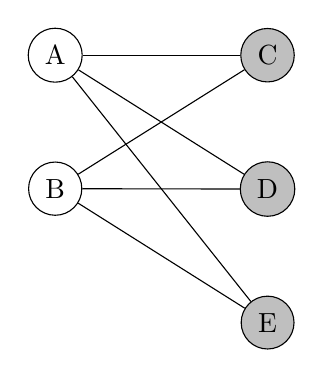
\begin{tikzpicture}[scale=1.3, auto,swap]
		\node[shape=circle,draw=black] (A) at (0,0) {A};
		\node[shape=circle,draw=black, below=of A] (B) {B};
		\node[shape=circle,draw=black,fill=lightgray, right= 2cm of A] (C) {C};
		\node[shape=circle,draw=black,fill=lightgray, below=of C] (D) {D};
		\node[shape=circle,draw=black,fill=lightgray, below=of D] (E) {E};
		
		\path [-] (A) edge (C);
		\path [-] (A) edge (D);
		\path [-] (A) edge (E);
		\path [-] (B) edge (C);
		\path [-] (B) edge (D);
		\path [-] (B) edge (E);		
		\end{tikzpicture}
	\end{figure}
	In der Regel wird nach einem möglichst großen Independent Set gesucht.
\end{frame}

\begin{frame}{Vertex Cover}
	\vspace{-0.5cm}
	\begin{block}{Definition}
		Gegeben einen Graphen $G$. Ein Vertex Cover $VC$ ist eine Menge von Knoten, sodass jede Kante in $G$ mit mindestens einem Knoten aus $VC$ verbunden ist.
	\end{block}

	\begin{figure}
		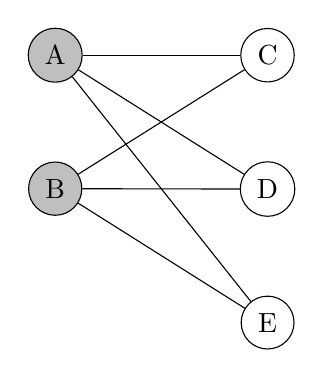
\begin{tikzpicture}[scale=1.3, auto,swap]
		\node[shape=circle,draw=black,fill=lightgray] (A) at (0,0) {A};
		\node[shape=circle,draw=black,fill=lightgray, below=of A] (B) {B};
		\node[shape=circle,draw=black, right= 2cm of A] (C) {C};
		\node[shape=circle,draw=black, below=of C] (D) {D};
		\node[shape=circle,draw=black, below=of D] (E) {E};
		
		\path [-] (A) edge (C);
		\path [-] (A) edge (D);
		\path [-] (A) edge (E);
		\path [-] (B) edge (C);
		\path [-] (B) edge (D);
		\path [-] (B) edge (E);		
		\end{tikzpicture}
	\end{figure}
	In der Regel wird nach einem möglichst kleinen Vertex Cover gesucht.
\end{frame}

\subsection{Sätze}
\begin{frame}{Zusammenhang zwischen \textbf{IS} und \textbf{VC}}
	\begin{block}{Satz}
		Sei $G=(V,E)$ eine Graph und $X\subseteq V$ eine Menge von Knoten. Dann gilt:
		\[X\text{ ist ein \textbf{VC} von $G$} \Longleftrightarrow V\setminus X\text{ ist ein \textbf{IS} von $G$}\]
	\end{block}
	\textbf{Beweis:}
	\begin{itemize}
		\item Sei $X$ ein beliebiges \textbf{VC}. Wir behaupten, dass $V\setminus X$ ein IS ist.
		\item Nehmen wir also das Gegenteil an und führen dies zum Widerspruch:
		\begin{itemize}
			\item Angenommen es würde $\{u,v\}\subseteq V\setminus X, u\neq v$ existieren mit $(u,v)\in E$
			\item Dann wäre aber $u,v\notin X$ und die Kante $(u,v)$ wäre vom VC $X$ nicht abgedeckt $\Rightarrow$ Widerspruch!
		\end{itemize}
		\item Die andere Richtung folgt ähnlich
	\end{itemize}
\end{frame}
\begin{frame}{Größe von \textbf{IS} und \textbf{VC}}
	\begin{block}{Definition}
		Ein \textbf{IS}/\textbf{VC} ist \textbf{inklusions maximal/minimal}, wenn kein Knoten hinzugefügt/entfernt werden kann ohne die Eigenschaft des \textbf{IS}/\textbf{VC} zu behalten.\\
		Ein \textbf{IS}/\textbf{VC} ist \textbf{kardinalitäts maximal/minimal}, wenn kein größeres/kleineres \textbf{IS}/\textbf{VC} existiert.
	\end{block}
	\begin{block}{Bemerkung}
		Ein kardinalitätsmaximales \textbf{IS} oder ein kardinalitätsminimales \textbf{VC} auszurechnen is $NP$-schwer.
	\end{block}
\end{frame}
\begin{frame}{Satz von König}
	\begin{block}{Satz (von Dénes König)}
		In einem bipartiten Graphen ist die Größe eines kardinalitätsminimalem Vertex Cover (\textbf{VC}) gleich der Größe eines Max Cardinality Bipartite Matching (\textbf{MCBM}).
	\end{block}
	Etwas informeller aufgeschrieben erhalten wir damit $|VC| = |MCBM|$.\\
	Und mit unserem Wissen aus dem vorangegangenen Satz folgt: $|V| = |VC| + |IS| = |MCBM| + |IS|$\\
\end{frame}

\begin{frame}{Guardian of Decency}
	\vspace{-0.3cm}
	\begin{block}{Aufgabe}
		Gegeben sind $N$ Schüler, beschrieben durch Größe, Geschlecht und Musikgeschmack. Der Lehrer möchte wissen wie viele Schüler maximal auf Klassenfahrt kommen können, ohne dass die Gefahr besteht, dass zwei Schüler ein Paar werden.\\
		Zwei Schüler laufen Gefahr ein Paar zu werden, wenn sie ein unterschiedliches Geschlecht, maximal 40cm Größendifferenz und einen gleichen Musikgeschmack haben.
	\end{block}
	\begin{itemize}
		\setlength\itemsep{0.05em}
		\item Modelliere das Problem als Graphen mit den Schülern als Knoten
		\item Verbinde Schüler, wenn sie ein Paar werden könnten
		\item Suche nach einem maximalem \textbf{IS}
		\item nutze dafür aus, dass der Graph bipartit ist, indem Männchen und Weibchen voneinander getrennt werden
		\item Berechne mittels Flow $|V|-|MCBM|=|V|-|VC|=|IS|$
	\end{itemize}
\end{frame}

\appendix
%\beginbackup

%\begin{frame}[allowframebreaks]{References}
%\printbibliography
%\end{frame}

%\backupend

\end{document}
